
\chapter{Introduction}

Modern optimising compilers have reached a high level of sophistication, providing a large number of optimisations.
Because of the unpredictability of optimisation interactions, in addition to the growing complexity of processor architectures and applications, the correct choice of optimisations and their ordering can have a significant impact on the performance of the code being optimised~\citep{pan06,fursin07,kulkarni12}.

Each of these optimisations interacts with the code in complicated ways, depending on all other optimisations and the order they were applied to the code being optimised.
Understanding the interactions of optimisations is very important in determining a good solution to the phase-ordering problem~\citep{touati06,kulkarni12}.
Because of all those dependencies and interactions, although most compiler optimisations yield significant improvements in many programs, the potential for performance degradation in certain program patterns is known to compiler writers and many users~\citep{pan06,zhou12,kulkarni12}.
%Traditional compilers typically apply the same set of optimisation in a fixed order to all functions in a program, without regard the code being optimised.

Efficiently selecting the best combination of compiler optimisations for a given program or program section remains an open problem.
Compiler writers typically use a combination of experience and insight to construct the default sequences of prearranged optimisations found in compilers.
However, these default pre-arranged set of optimisations do not include all possible optimisations and they are always applied in the same pre-defined fixed order, without regard the code being optimised~\citep{pan06,cavazos07,zhou12,kulkarni12}.
%in hopes that a programmer will know which combination of optimisations will benefit their code~\cite{pan06,cavazos07,zhou12,kulkarni12}.

A well known compilation technique that addresses this challenge is {\itercomp}.
{\Itercomp} has the ability to adapt to new platforms, program and workload while still having a systematic and simple optimisation process.
It works by repeatedly evaluating a large number of compiler optimisations until the best combination is found for a particular program~\citep{fursin07,chen10}.
The main challenge concerning {\itercomp} is the need for efficiently exploring such a large optimisation space~\citep{fursin07,cavazos07,zhou12}.

Until recently, most of existing work  had been focusing on finding the best optimisation through repeated runs using a single input.
Although they demonstrate the potential of {\itercomp}, in real scenarios the user rarely executes the same input dataset multiple times~\citep{bodin98,kisuki99,stephenson03,kulkarni04,agakov06}.
Applying {\itercomp} in light of a single input may not result in good performance when executing the optimised code with different inputs.

Most of real world applications are complex enough so that a single input case does not capture the whole range of possible scenarios and program behaviour~\citep{haneda06,fursin07,chen10,chen12a}.
Because programs can exhibit behaviours that differ greatly depending on the input,
%This is something that is well known when writing test cases for correctness.
%We can extend the same argument when optimising the code for performance.
using a single input for {\itercomp} can produce poor performance when executed with different inputs.

Recent work have been studying the impact of using multiple input datasets
for performing {\itercomp}.
This previous work suggests that optimising based on a representative range of input datasets allows for selecting a robust compiler optimisation that produces good performance in real scenarios where the input is expected to change constantly~\citep{haneda06,fursin07,chen10,chen12a,chen12b,fang15,mpeis16}.
Their results show that a limited number of input datasets may be sufficient to obtain a well optimised program for a wider range of different inputs~\citep{haneda06,fursin07,chen10,chen12a}.

Finding such a robust combination of compiler optimisations by means of {\itercomp} across a large range of inputs may be very time consuming.
In order to speed up this process we intend to reduce the number of actual executions during the exploration of the optimisation space without much degradation of the final selected optimisation.

\begin{figure}[htb]
    \centering
    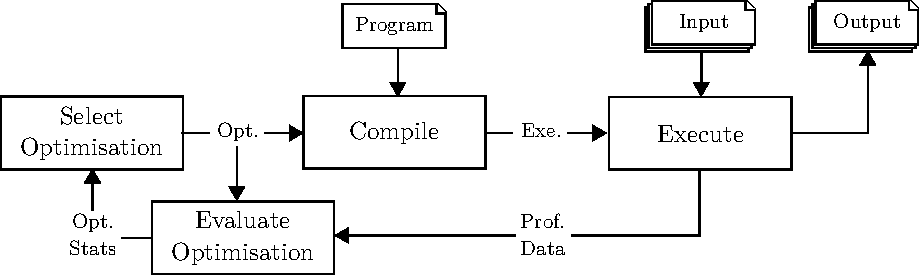
\includegraphics[width=\linewidth]{figs/diagram}
    \caption{Overview of the execution engine for applying {\itercomp}.}
    \label{fig:diagram}
\end{figure}

In this work, our main goal is to enable {\itercomp} in \textit{online} scenarios with the restriction of executing distinct inputs only once, while targeting optimal performance across different inputs.
This online aspect is usually found in mobile and data centre platforms~\citep{chen12b,fang15,mpeis16}, where the goal is to optimise programs based on the workload of a particular user (or group of users) between executions.

Measuring just execution time, for example, is useful only if the amount of work is constant between executions with different inputs.
For this reason, we propose the use of a work-based metric in order to compare the performance of different optimisations across multiple executions of the program with distinct inputs.

Because of the restriction of not repeating inputs, we instrument the program for measuring the amount of work it performed during its execution.
Having a low overhead instrumentation is essential in this online scenario for two main reasons:
$(i)$ the user is directly affected by large overheads;
$(ii)$ a highly intrusive instrumentation can havea significant impact on the effect of the optimisations.

Our main contributions are the following:
\begin{itemize}
\item The use of a work-based performance metric in order to enable \textit{online} {\itercomp} by comparing different combination of compiler optimisations even when executed with distinct inputs.
\item We propose a relaxed instrumentation for low overhead profiling, with a controlled trade-off between accuracy and overhead.
\end{itemize}

